% Sample LaTeX file for creating a paper in the Morgan Kaufmannn two
% column, 8 1/2 by 11 inch proceedings format.

\documentclass[letterpaper]{article}
\usepackage{uai2019}
\usepackage[margin=1in]{geometry}

% Set the typeface to Times Roman
\usepackage{times}

\usepackage{algorithm,algorithmic}
\newcommand{\theHalgorithm}{\arabic{algorithm}}

\usepackage{microtype}
\usepackage{graphicx}
\usepackage{subfigure}
\usepackage{booktabs} % for professional tables

\usepackage{natbib}

\usepackage{amssymb} %maths
\usepackage{amsmath} %maths
\usepackage{amsthm}
\usepackage{hyperref}
\usepackage[utf8]{inputenc} %useful to type directly diacritic characters
\usepackage[capitalize]{cleveref}
\crefname{prop}{Proposition}{Propositions}
\crefname{thm}{Theorem}{Theorems}
\crefname{lem}{Lemma}{Lemmas}
\crefname{algorithm}{Algorithm}{Algorithms}

\def\rva{{\mathbf{a}}}
\def\rvo{{\mathbf{o}}}
\def\rvr{{\mathbf{r}}}
\def\rvs{{\mathbf{s}}}
\def\rvu{{\mathbf{u}}}
\def\rvw{{\mathbf{w}}}
\def\rvx{{\mathbf{x}}}
\def\rvg{{\mathbf{g}}}
\def\rvo{{\mathbf{o}}}
\def\rvone{{\mathbf{1}}}
\def\rvzero{{\mathbf{0}}}
\def\rvtilder{{\tilde{\mathbf{r}}}}
\def\rvhat{{\hat{\mathbf{r}}}}

\def\rvp{{\mathbf{p}}}

\def\pr{{\text{Pr}}}
\def\r{{\text{R}}}

\def\regret{{\text{Regret}}}

\newtheorem{thm}{Theorem}
\newtheorem{lem}{Lemma}
\newtheorem{defi}{Definition}
\newtheorem{prop}{Proposition}
\newtheorem{remk}{Remark}

\def\rvpi{{\boldsymbol{\pi}}}

\def\rmA{{\mathbf{A}}}
\def\rmD{{\mathbf{D}}}
\def\rmI{{\mathbf{I}}}
\def\rmW{{\mathbf{W}}}
\def\rmX{{\mathbf{X}}}

\def\sE{{\mathbb{E}}}
\def\sR{{\mathbb{R}}}
\def\sI{{\mathbb{I}}}
\def\sP{{\mathbb{P}}}

\def\gN{{\mathcal{N}}}
\def\gE{{\mathcal{E}}}
\def\gU{{\mathcal{U}}}

\DeclareMathOperator*{\argmax}{arg\,max}
\DeclareMathOperator*{\argmin}{arg\,min}
\DeclareMathOperator*{\probability}{Pr}
\DeclareMathOperator*{\expectation}{\sE}

\title{On Optimal Stochastic Bandit Algorithms and Provable Policy Gradient Methods with Neural Networks}

\author{} % LEAVE BLANK FOR ORIGINAL SUBMISSION.
          % UAI  reviewing is double-blind.

% The author names and affiliations should appear only in the accepted paper.
%
%\author{ {\bf Harry Q.~Bovik\thanks{Footnote for author to give an
%alternate address.}} \\
%Computer Science Dept. \\
%Cranberry University\\
%Pittsburgh, PA 15213 \\
%\And
%{\bf Coauthor}  \\
%Affiliation          \\
%Address \\
%\And
%{\bf Coauthor}   \\
%Affiliation \\
%Address    \\
%(if needed)\\
%}

\begin{document}

\maketitle

\begin{abstract}
In this paper, we propose a deep reinforcement learning algorithm which achieves nearly optimal finite time regret in the stochastic bandit setting. In our method, the agent maintains its action selection strategy in a parametric fashion. After enough exploration, a neural network is trained to minimized the empirical value related objectives using gradient updates. The policy is obtained from the exponential weight of learned logits. While our method is unlike standard bandit algorithms which directly utilize statistics from samples, we show that its finite time regret is nearly optimal up to log and constant factor. The results can be generalized to episodic MDPs and the state dependent bandit cases.
\end{abstract}

\section{Introduction}
\label{introduction}

Deep Reinforcement Learning (DRL) has recently achieved great successes, including games \citep{silver2016masteringA,silver2017masteringB,moravvcik2017deepstack,mnih2015human}, robotics \citep{lillicrap2015continuous,levine2016end}, just name a few. However, comparing with its brilliant achievements, the theoretical understanding of the mechanism behind DRL methods is not enough to explain its practical performance. 

DRL combines techniques in Deep Learning (DL) and Reinforcement Learning (RL) fields, to understand DRL, we need findings from both the DL and the RL sides.

On the RL side, it is well studied that under the bandit settings, and the tabular cases of the Markov decision process (MDP) setting, a number of algorithms enjoy favorable theoretical guarantees \citep{bubeck2012regret,sutton2018reinforcement}. In particular, either the optimal policies can be learned asymptotically, or within finite time, sublinear regret can be obtained. However, once it goes beyond the tabular cases, the theoretical results become much weaker. For example, Gradient Temporal Difference (GTD) with (non-)linear function approximations can only converge to the fixed points of projected Bellman operators \citep{sutton2009fast,sutton2009convergent,bhatnagar2009convergent}. While the performance of the fixed point policies can be arbitrarily bad without any further assumptions on the function approximations.

On the DL side, the empirical achievements are also much more advanced than the  theoretical results \citep{goodfellow2016deep}. However, there are still progresses in the expressiveness, optimization, and generalization aspects of DL theory. In particular, very recently, it has been discovered that, in supervised learning (regression and classification) settings, the training loss can be globally optimized (in linear convergence rate for $\ell_2$ loss in regression, and in constant time for classification) by gradient descent (GD) and stochastic gradient descent (SGD) method, given that the number of parameters in hidden layer is quite large, i.e., overparameterization. With some additional structured data distribution assumptions, the convergent training loss can be generalized to testing loss, making the neural network have provable generalization ability. 

To combine progresses in the DL and RL fields, we consider two main diferences between RL and supervised learning: (a) unlike the supervised learning settings, there are no true labels when learning RL agents; (b) to learn good agents, enough exploration is necessary.

In this paper, based on the recent progresses in overparameterized neural network optimization, we make one step forward to theoretically understanding DRL. In particular, we make the following contributions.
\begin{itemize}
    \item We prove that in bandit setting, with enough exploration, the widely-used policy gradient method, with policy net represented by a overparameterized two layer neural network (NN), achieves $O\left( \sqrt{T} \right)$ regret.
    \item We show that in episodic MDP setting, with the same exploration strategy and policy net as above, policy gradient method achieves $O\left( \sqrt{T} \right)$ regret.
    \item In many state dependent bandit and MDP settings, similar results also hold.
\end{itemize}

We would like to point that the above results can be generalized to policy net represented by multi-layered neural networks. Assuming a two layer NN policy is just for simplicity and conciseness. We provide the generalization to multi-layered NN in the appendix for completeness.

To our knowledge, our finding is the first convergence result for popular RL methods (here, policy gradient) with non-linear NN function approximations, which provides theoretical support for DRL methods. Our result is just beginning of understanding many other DRL methods (such as DQN \cite{mnih2015human}, A3C \citep{mnih2016asynchronous}, and PCL \citep{nachum2017bridging}), with more practical NN function approximations (e.g., less overparameterized), using many other policy optimization techniques (such as mirror descent, and relative entropy policy search).

The rest of the paper is organized as follows. Some proofs are deferred to appendix due to space limit.

\subsection{Notations}

Bold letters refer to vectors, and non-bold letters refer to scalars. For example, $u_{i,r} \in \sR$ is the $r$th component of vector $\rvu_i \in \sR^m$. $n$ is the total number of states, while $m$ is the total number of nodes in each hidden layer. $h$ is the total number of actions can be taken at each state. $\rvone$ means all-one vector, and $\rmI$ refers to identity matrix, with dimensions depends on the contexts.

Denote $[n] \triangleq \left\{ 1,2, \dots, n \right\}$. $\rvs_i \in \sR^d$, $i \in [n]$ refers to a state. $\rvw_r \in \sR^d$, $r \in [m]$ is a weight vector in the first hidden layer. $\rmW^\top \triangleq \left[ \rvw_1, \rvw_2, \dots, \rvw_m \right] \in \sR^{d \times m}$ is the weight matrix of the first hidden layer. $u_{i,r} \triangleq \rvw_r^\top \rvs_i$ is the $r$th node value of the first hidden layer. $\rva_k \in \sR^m$, $k \in [h]$ is a weight vector in the second hidden layer. In the paper, after the random initialization $\rva_k \sim \gU\left\{-1, +1\right\}$, $\rva_k$ will be fixed. This assumption is common in literature \citep{li2018learning,du2018gradientA,du2018gradientB,allen2018convergenceA,allen2018convergenceB}, and has been empirically verified that has no impact on the performance of trained neural networks \citep{hoffer2018fix}. Other initialization like $\rva_k \sim \gN(0, \rmI)$ also works. $\rmA^\top \triangleq \left[ \rva_1, \rva_2, \dots, \rva_h \right] \in \sR^{m \times h}$ is the weight matrix of the second hidden layer. $o_{i,k} \triangleq \sum\limits_{r=1}^{m}{a_{k,r} \cdot \sigma\left( u_{i,r} \right)}$ is the logit of the $k$th action for state $\rvs_i$, where $\sigma(\cdot) \triangleq \max\left\{ \cdot, 0 \right\}$ is the ReLU activation function. $\pi_{i,k} \triangleq f\left( o_{i,k} \right) \triangleq \frac{\exp\left\{ o_{i,k} \right\}}{\sum\limits_{k^\prime = 1}^{h}{\exp\left\{ o_{i,k^\prime} \right\}}}$ is the probability of choosing action $k$ at state $\rvs_i$, where $f(\cdot)$ is the softmax function. $\rvr_i \in \sR^h$ is the true reward vector at state $\rvs_i$. $\r_i^{\max} \triangleq \max\limits_{k \in [h]}\left\{ r_{i,k} \right\}$ is the maximum reward at state $\rvs_i$. $\rvtilder_i \triangleq \r_i^{\max} \cdot \rvone - \rvr_i$ is the true loss vector at state $\rvs_i$. Given stochastic policies $\rvpi \triangleq \left[ \rvpi_1, \rvpi_2, \dots, \rvpi_n \right] \in \sR^{h \times n}$, the expected loss is defined as,
\begin{equation}
\label{eq:expected_loss}
\begin{split}
    \ell \triangleq \frac{1}{n} \cdot \sum\limits_{i=1}^{n}{ \left( \r_i^{\max} - \rvpi_i^\top \rvr_i \right) } = \frac{1}{n} \cdot \sum\limits_{i=1}^{n}{ \rvpi_{i}^\top \rvtilder_{i} }.
\end{split}
\end{equation}

Without loss of generality, we assume $\rvr_i \in \left[ 0, 1 \right]^h$, $\forall i \in [n]$. Therefore $\rvtilder_i \in \left[ 0, 1 \right]^h$, $\forall i \in [n]$. For simplicity, we also assume $\rvr_i$ is a deterministic vector, $\forall i \in [n]$, while the results also generalize to random reward vectors. Finally, we use $\Delta_i \triangleq \max\limits_{k \in [h]}\left\{ \tilde{r}_{i,k} \middle| \tilde{r}_{i,k} > 0 \right\}$ to denote the reward gap between the optimal arm and the arm with the second largest reward at state $\rvs_i$, $\forall i \in [n]$.

\section{BACKGROUND}
\label{sec:background}

We focus on the stochastic bandit setting in this paper where the policy or the values of the actions are represented using a 2-layers neural networks.  
However, our results can be easily generalized to many other reinforcement learning settings, e.g. state dependent stochastic bandit settings and episodic MDP settings.

\subsection{STOCHASTIC BANDIT SETTINGS}
\label{subsec:settings}

One can think of that the standard stochastic bandit setting has only 1 state.  
At each time step $t$, the agent takes an action $A_t \in [h]$ according to its own strategies $\rvpi_t$, and then it observes a random reward $R_{A_t} \in \sR$, where the mean value of $R_{A_t}$ is $r_{A_t}$. 
The agent then improves its action selection strategies. 
After such $T$ time steps, the performance of the agent's strategy is measured by the (expected) regret,
\begin{equation}
\label{eq:expected_regret}
R_n = \sum\limits_{t=0}^{T-1}{{\rvpi^*}^\top \rvr} - \sE \left[ \sum\limits_{t=0}^{T-1}{  r_{ A_t}  } \right] 
%= \sum\limits_{t=0}^{T-1}{{\rvpi^*}^\top \rvr} - \sum\limits_{t=0}^{T-1}{ \sE \left[ r_{A_t} \right] },
\end{equation}
where the expectation is over the randomness of action selection, if the agent is using some stochastic strategies.
Obviously, $\rvpi^*$ is a one-hot vector and by standard calculation, one can show that
\[
R_n = \sum_a \sum_{t=1}^T \rvpi_t(a) \Delta(a),
\]
where $\Delta(a) = \max_b r(b)- r(a)$, $r(a)$ is the expected reward of the action $a$.

%\subsubsection{Episodic Markov decision process (MDP) (maybe remove this section)}
%The episodic MDP setting recovers the bandit setting as a special case. The environment randomly select a starting state $\rvs_i^0 \in \sR^d$. At each time step $t$, the agent takes one action $A_t \in [h]$ according to some strategies, and then it observes a reward $R_{i, A_t} \in \sR$ and next state $S_{t+1} \sim \sP\left( \cdot \middle| S_t, A_t \right)$, where $\sP$ is the transition probability matrix and it is unknown to the agent. After such $H$ steps, the agent observes an ending state $S_H$, and the current trajectory terminates. At the next time step, the agent will observe a new starting state $\rvs_i^0$ randomly generated by the environment. Since we use policy gradient method (no value learning), the agent updates its NN policy weights using the cumulative reward collected after each single trajectory terminates.

\begin{figure}[t]
	\vskip 0.2in
	\begin{center}
		\centerline{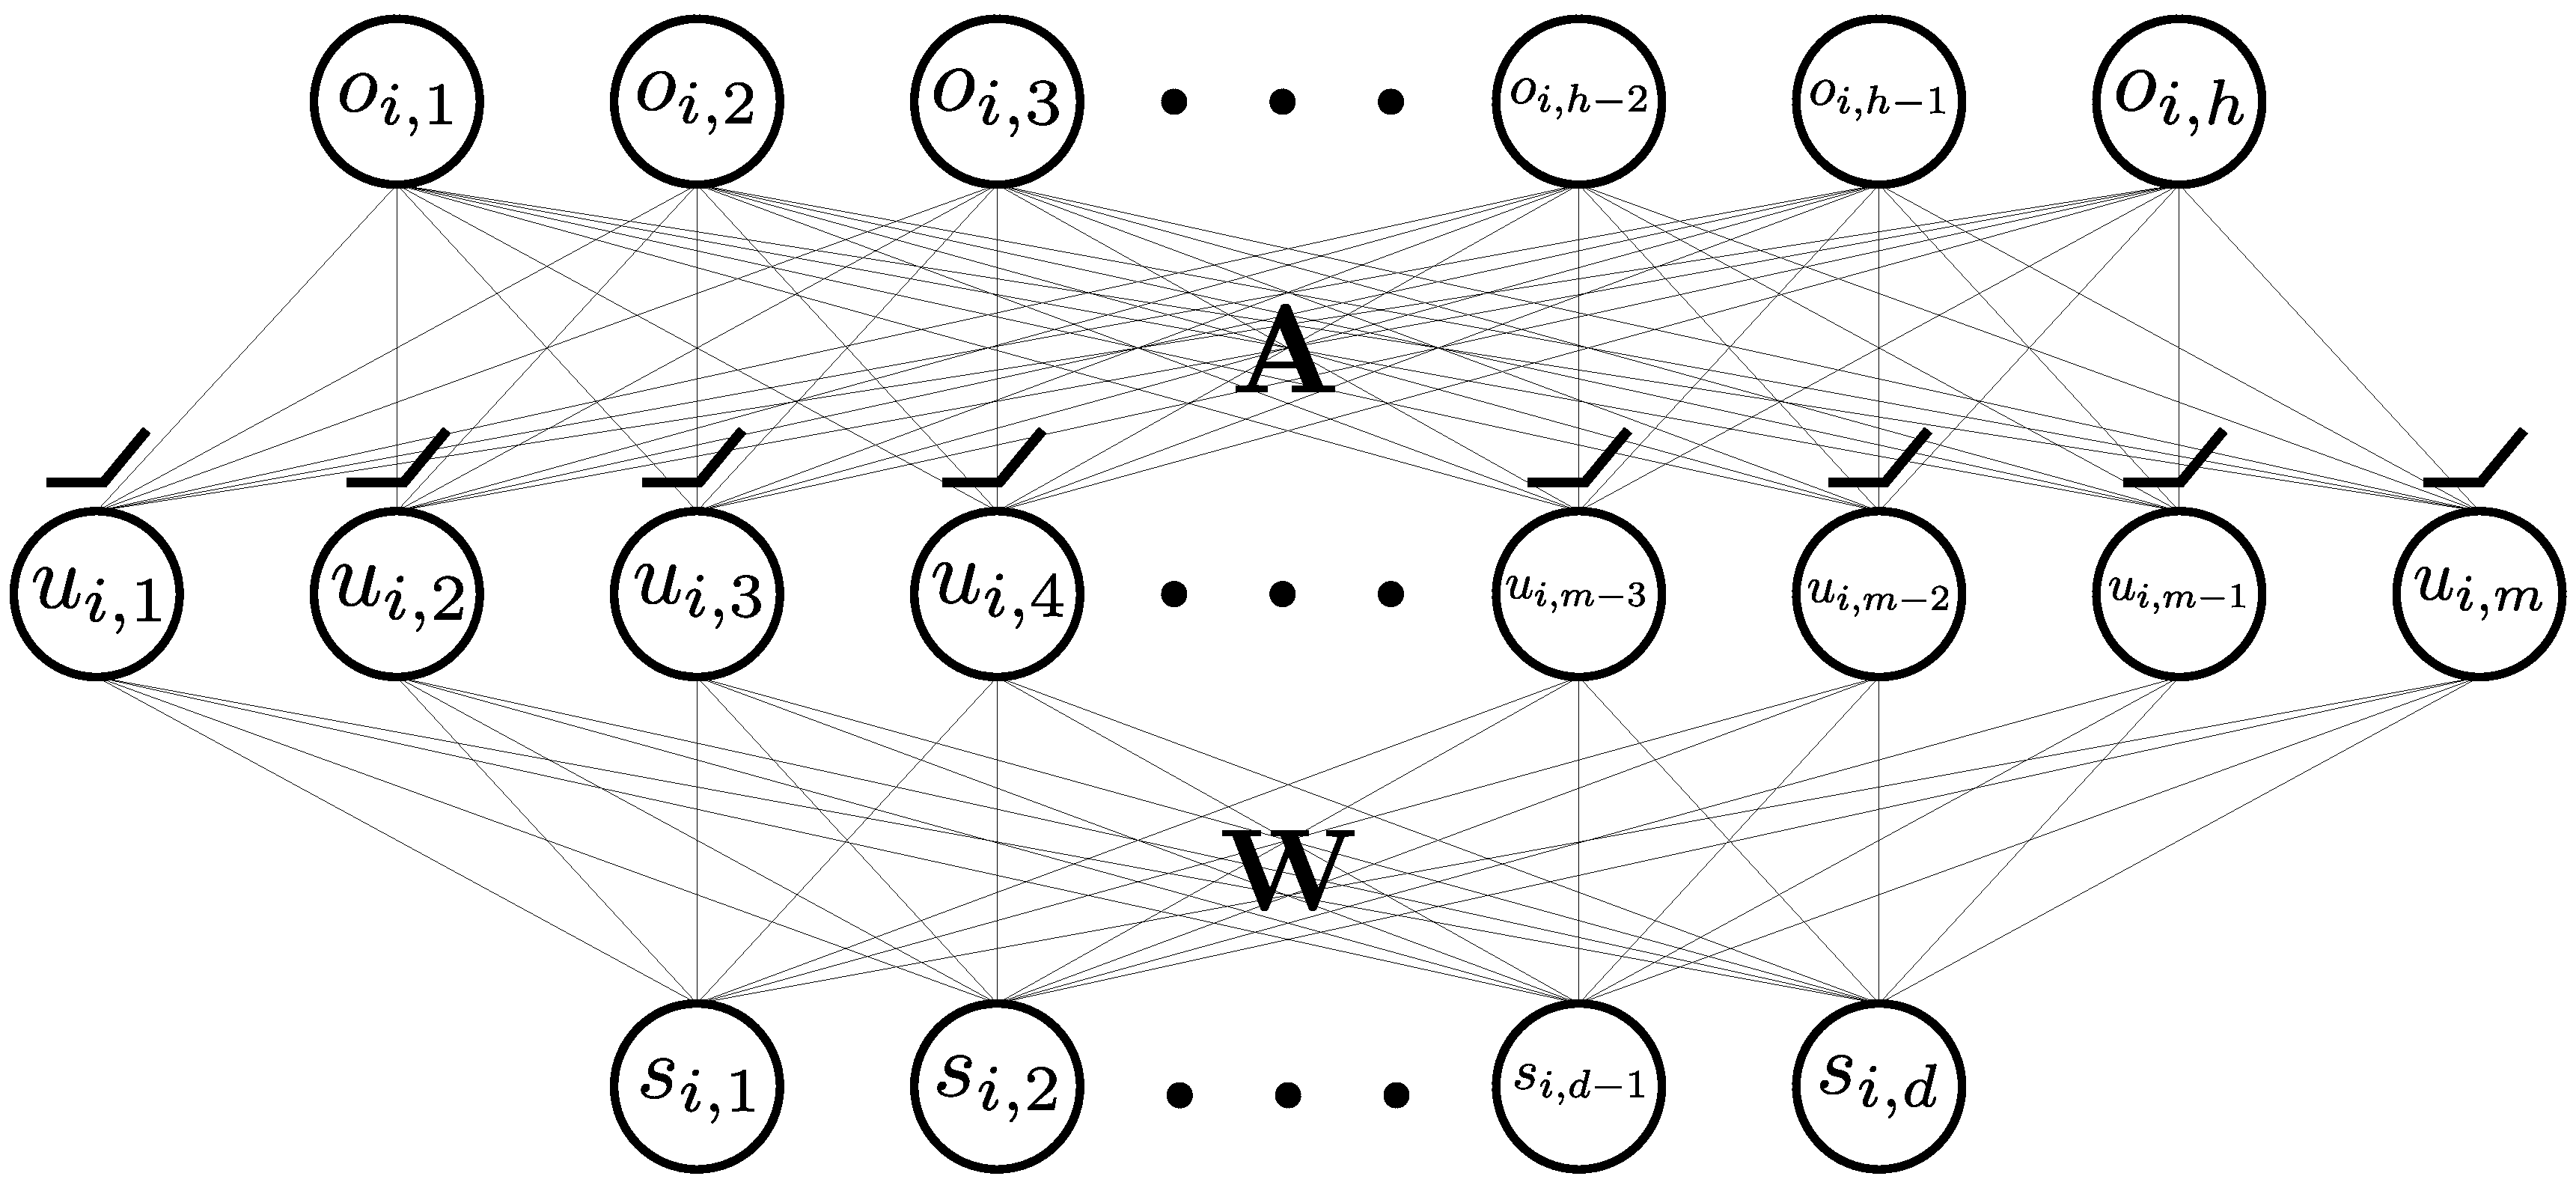
\includegraphics[width=\columnwidth]{nn_value.pdf}}
		\caption{Value neural network.}
		\label{fig:nn_value}
	\end{center}
	\vskip -0.2in
\end{figure}



%We mainly focus on the standard stochastic bandit setting with $n = 1$, i.e., there is only one state $\rvs_i$. At each time step $t$, the agent takes an action $A_t \in [h]$ according to its own strategies, and then it observes a random reward $R_{i, A_t} \in \sR$, where the mean value of $R_{i, A_t}$ is $r_{i, A_t}$. The agent then uses the reward to improve its action selection strategies. After such $T$ time steps, the performance of the agent's strategy is measured by the (expected) regret,
%\begin{equation}
%\label{eq:expected_regret}
%    \sum\limits_{t=0}^{T-1}{{\rvpi_i^*}^\top \rvr_i} - \sE \left[ \sum\limits_{t=0}^{T-1}{  r_{i, A_t}  } \right] = \sum\limits_{t=0}^{T-1}{{\rvpi_i^*}^\top \rvr_i} - \sum\limits_{t=0}^{T-1}{ \sE \left[ r_{i, A_t} \right] },
%\end{equation}
%where the expectation is over the randomness of action selection, if the agent is using some stochastic strategies.


\subsection{NEURAL NETWORK VALUE FUNCTION APPROXIMATION AND POLICY}
\label{subsec:nn_value_policy}
The structure of the value network and the policy network  is a 2-layers fully connected neural network with ReLU activation, as shown in \cref{fig:nn_value} and \cref{fig:nn_policy}, respectively. 
Each neural network takes the state $\rvs \in \sR^d$ as its input, where without loss of generality we assume that $\left\| \rvs \right\|_2 = 1$.
The hidden layer of both networks are denoted by $\rvu   \triangleq W\rvs\in\sR^m$, and the logit output $\rvo \triangleq A\sigma\left( \rvu\right) \in \sR^h$, where $\sigma$ is element-wise ReLU activation function. 
The policy network differs the value network with one additional softmax transform layer in order to output probability distributions, where $\rvpi \triangleq f\left( \rvo \right) = f\left( \rmA \sigma\left( \rmW \rvs \right) \right)$, and $f$ is the softmax function. In the rest of the paper we denote the policy $\rvpi$ by $\rvpi(\rmW)$ to emphasize its parametrization by $\rmW$. 

%Both the value and the policy neural networks take the state feature  $\rvs_i \in \sR^d$ as the input. Then the networks calculate the hidden node value vector by $u_{i,r} \triangleq \rvw_r^\top \rvs_i$, $\forall r \in [m]$. The logit vector is then calculated by $o_{i,k} \triangleq \rva_k^\top \sigma\left( \rvu_i \right)$, $\forall k \in [h]$, where $\sigma$ is element-wise ReLU activation function. The value neural network outputs the logit vector $\rvo_i$. While the policy neural network output probability is the softmax transform of the logit vector, i.e., $\rvpi_i \triangleq f\left( \rvo_i \right) = f\left( \rmA \sigma\left( \rmW \rvs_i \right) \right)$. 

\begin{figure}[t]
\vskip 0.2in
\begin{center}
\centerline{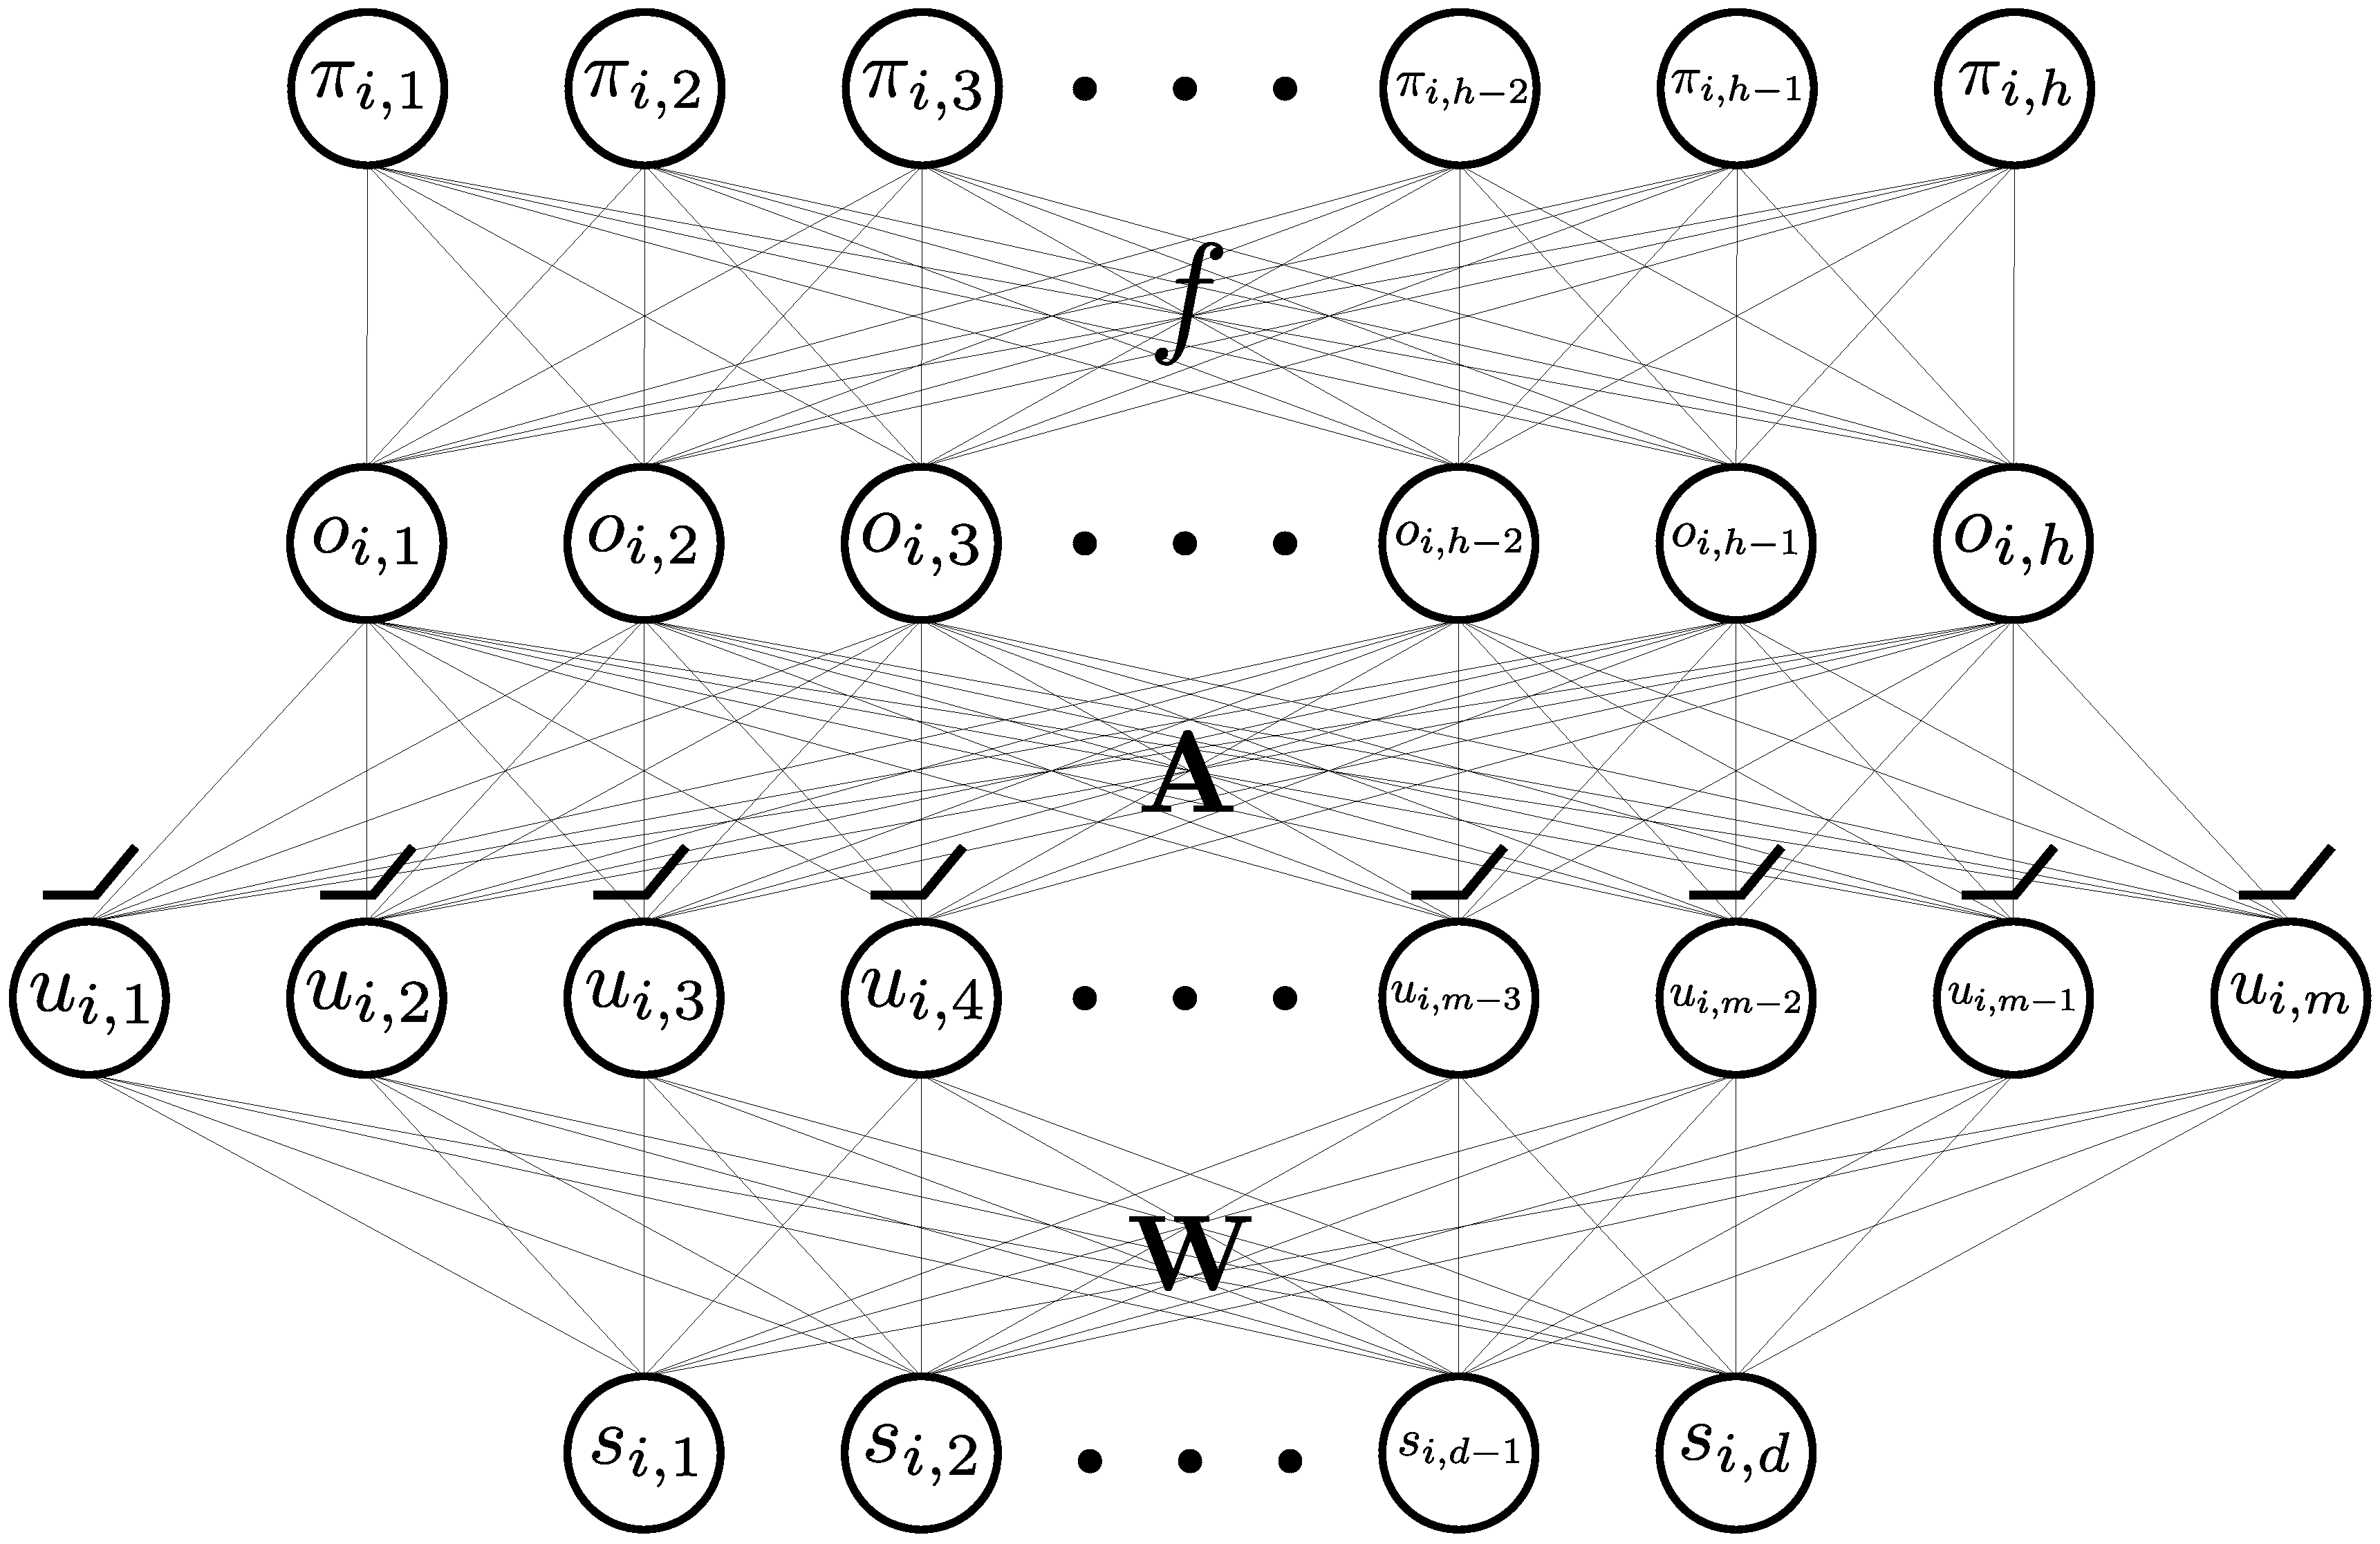
\includegraphics[width=\columnwidth]{nn_policy.pdf}}
\caption{Policy neural network.}
\label{fig:nn_policy}
\end{center}
\vskip -0.2in
\end{figure}

%The policy neural network defines a family of policies $\rvpi_i \left( \rmW \right)$ parameterized by $\rmW \in \sR^{m \times d}$ given any state $\rvs_i$. Let $\rvpi_i = \rvpi_i \left( \rmW \right)$, the expected loss of the policy neural network can be calculated according to \cref{eq:expected_loss}.

\paragraph{Multi-layered neural networks.} We would like to point that our algorithms and results can be easily extended to general value functions and policies parameterized by multi-layered neural networks \citep{allen2018convergenceA,allen2018convergenceB,du2018gradientA}. For the sake of simplicity and conciseness, we focus on two-layers neural networks in the paper.

%Although there is only one state, i.e., $n = 1$, and $i$ can be omitted without ambiguity, we choose to keep the subscript $i$ here to make the generalization from the standard bandit setting to the many state dependent setting smoother, and our algorithms work for general $n > 1$. For simplicity, we assume $\left\| \rvs_{i} \right\|_2 = 1$, $\forall i \in [n]$.

%In the case of $n > 1$, for each state $\rvs_i$, there is a state dependent policy $\rvpi_i$. And the agent's goal is to learn totally $n$ policies using only one neural network. We assume $\left\| \rvs_{i} -  \rvs_{j} \right\|_2 \ge \delta > 0 , \ \forall i \not= j$, i.e., no duplicated data, and $\left\| \rvs_{i} \right\|_2 = 1, \ \forall i \in [n]$.

\subsection{LOGIT LEARNING}
\label{subsec:logit_learning}

Our first proposed algorithm is Logit Learning with $\epsilon$-Greedy Exploration, as shown in \cref{alg:logit_learning_eps_greedy_exploration}. After the random initialization, at each time step $t$, the agent selects the action with the largest logit with probability $1 - \epsilon_t$, and it uniformly randomly select actions with the other probability $\epsilon_t$. After taking action and observing rewards, the agent improves its strategies by minimizing the value loss objective $\frac{1}{2} \left\| \rvo_i\left( \rmW\left(t\right)\right) - \hat{\rvr}_i\left(t\right) \right\|_2^2$, where $\hat{\rvr}_i\left(t\right)$ is the empirical mean reward estimated from sampled rewards up to step $t$. In each iteration, the agent only update its value neural network using one gradient descent, therefore the logit learning is in an online fashion.


\begin{algorithm}[t]
   \caption{Logit Learning with $\epsilon$-Greedy Exploration}
\label{alg:logit_learning_eps_greedy_exploration}
\begin{algorithmic}
   \STATE {\bfseries Input:} State feature $\rvs_i$, learning rate $\eta > 0$.
   \STATE $\rvw_r(0) \sim \gN\left( 0, \sigma^2 \cdot \rmI \right)$, $\forall r \in [m]$.
   \STATE $a_{k, r} \sim \gU\left\{-1, +1\right\}$, $\forall k \in [h]$, $\forall r \in [m]$.
   \STATE $\hat{r}_{i,k}\left(0\right) \gets 0$, $n_{i,k}\left(0\right) \gets 0$, $\forall k \in [h]$.
   \STATE $\hat{\Delta}_{i,k}\left(0\right) \gets \max\limits_{k^\prime}\left\{ \hat{r}_{i,k^\prime}\left(0\right) \right\} - \hat{r}_{i,k}\left(0\right)$, $\forall k \in [h]$.
   \STATE $\tilde{\Delta}_{i,k}\left(0\right) \gets \max\limits_{k^\prime}\left\{ o_{i,k^\prime}\left(0\right) \right\} - o_{i,k}\left(0\right)$, $\forall k \in [h]$.
   \FOR{$t=0$ {\bfseries to} $T-1$}
   \STATE $\xi_t \gets \frac{\log{t}}{t \hat{\Delta}_{i,k}^2\left(0\right)}$, $\epsilon_t \gets \min\left\{ \frac{1}{2 h}, \xi_t \right\}$.
   \STATE $\pi_{i, k}\left(t\right) \gets 1$, for $k = \argmax\limits_{k^\prime \in \left[h\right]}\left\{ o_{i, k^\prime}\left(t\right)\right\}$.
   \STATE $\pi_{i, k}\left(t\right) \gets 0$, $\forall k \not= \argmax\limits_{k^\prime \in \left[h\right]}\left\{ o_{i, k^\prime}\left(t\right)\right\}$.
   \STATE $\tilde{\rvpi}_i\left(t\right) \gets \left( 1 - \epsilon_t \right) \cdot  \rvpi_i\left(t\right) + \epsilon_t \cdot \gU{\left[ h \right]}$.
   \STATE Sample action $A_{t} \sim \tilde{\rvpi}_{i}\left(t\right)\left(\cdot \middle| \rvs_i \right)$.
   \STATE Take action $A_{t}$. Observe reward $R_{i, A_{t}}\left(n_{i, A_{t}}\left(t\right) \right)$.
   \STATE $n_{i, A_{t}}\left(t+1\right) \gets n_{i, A_{t}}\left(t\right) + 1$.
   \STATE $\hat{r}_{i,A_{t}}\left(t+1\right) \gets \frac{n_{i, A_{t}}\left(t\right) \cdot \hat{r}_{i,A_{t}}\left(t\right) + R_{i, A_{t}}\left(n_{i, A_{t}}\left(t\right)\right) }{n_{i, A_{t}}\left(t+1\right)}$.
   \STATE $n_{i, k}\left(t+1\right) \gets n_{i, k}\left(t\right)$, $\forall k \not= A_t$.
   \STATE $\hat{r}_{i,k}\left(t+1\right) \gets \hat{r}_{i,k}\left(t\right)$, $\forall k \not= A_t$.
   \STATE $\rmW(t+1) \leftarrow \rmW(t) - \eta \cdot \frac{d \left\{ \frac{1}{2} \left\| \rvo_i\left( \rmW\left(t\right)\right) - \hat{\rvr}_i\left(t\right) \right\|_2^2 \right\}}{d \rmW(t)}$.
   \ENDFOR
\end{algorithmic}
\end{algorithm}

\subsection{POLICY GRADIENT}
\label{subsec:policy_gradient}

Our second proposed algorithm is based on the widely used policy gradient method. Consider at each step $t$, the agent is using $\rvpi_i\left(\rmW(t)\right)$ as shown in \cref{fig:nn_policy} as its action selection strategy, then the (expected) regret is equivalent to the cumulative expected loss of $\rvpi_i\left(\rmW(t)\right)$, i.e., 
\begin{equation}
\label{eq:vanilla_policy_gradient_expected_regret}
\begin{split}
    &\sum\limits_{t=0}^{T-1}{{\rvpi_i^*}^\top \rvr_i} - \sum\limits_{t=0}^{T-1}{ \expectation\limits_{A_t \sim \rvpi_i\left(\rmW(t)\right)} \left[ r_{i, A_t} \right] } \\
    &= \sum\limits_{t=0}^{T-1}{{\rvpi_i^*}^\top \rvr_i} - \sum\limits_{t=0}^{T-1}{\rvpi_i\left(\rmW(t)\right)^\top \rvr_i},
\end{split}
\end{equation}
by \cref{eq:expected_loss} and \cref{eq:expected_regret}. Using \cref{eq:vanilla_policy_gradient_expected_regret}, at each time step $t$, the agent can use the current NN policy $\rvpi_i\left(\rmW(t)\right)$ to sample an action, and obtain an estimation of the expected loss $\rvpi_i\left(\rmW(t)\right)^\top \rvr_i$. Doing policy gradient updates with respect to the NN weights $\rmW(t)$ will arguably decrease the expected loss, thus reduce the expected regret. 

Unfortunately, the vanilla policy gradient often suffers the ``lack of exploration" problem in practice, i.e., some actions can never be explored thus cannot be learned. Therefore, we propose a two stage algorithm combining policy gradient with uniform exploration as shown in \cref{alg:policy_gradient_uniform_exploration}. After the random initialization, at each step $t$, one of the two cases happens. If $t < T^{\frac{2}{3} + \beta}$, then agent gets into a purely ``exploring phase", without learning the policy neural network, while just collecting empirically estimated rewards. If $t \ge T^{\frac{2}{3} + \beta}$, then the agent starts ``playing and learning". The agent samples and takes actions according to the current neural network policy $\rvpi_{i}\left(\rmW(t)\right)$. In the meanwhile, the agent learns the policy neural network by doing policy gradient updates, with the expected empirically estimated loss calculated from the exploring phase as its objective.

\begin{algorithm}[t]
   \caption{Policy Gradient with Uniform Exploration}
\label{alg:policy_gradient_uniform_exploration}
\begin{algorithmic}
   \STATE {\bfseries Input:} State feature $\rvs_i$, learning rate $\eta > 0$, $\beta > 0$.
   \STATE $\rvw_r(0) \sim \gN\left( 0, \sigma^2 \cdot \rmI \right)$, $\forall r \in [m]$.
   \STATE $a_{k, r} \sim \gU\left\{-1, +1\right\}$, $\forall k \in [h]$, $\forall r \in [m]$.
   \STATE $\hat{r}_{i,k}\left(0\right) \gets 0$, $n_{i,k}\left(0\right) \gets 0$, $\forall k \in [h]$.
   \FOR{$t=0$ {\bfseries to} $T-1$}
   \IF{$t < T^{\frac{2}{3} + \beta}$}
   \STATE (Exploring Phase)
   \STATE Uniformly randomly sample action $A_{t} \in [h]$.
   \STATE $\rmW(t+1) \leftarrow \rmW(t)$.
   \ELSE
   \STATE (Playing-Learning Phase)
   \STATE Sample action $A_{t} \sim \rvpi_{i}\left(\rmW(t)\right)\left(\cdot \middle| \rvs_i \right)$.
   \STATE $\rmW(t+1) \leftarrow \rmW(t) + \eta \cdot \frac{d \rvpi_{i}\left(\rmW(t)\right)^\top \hat{\rvr}_i \left(t\right)}{d \rmW(t)}$.
   \ENDIF
   \STATE Take action $A_{t}$. Observe reward $R_{i, A_{t}}\left(n_{i, A_{t}}\left(t\right) \right)$.
   \STATE $n_{i, A_{t}}\left(t+1\right) \gets n_{i, A_{t}}\left(t\right) + 1$.
   \STATE $\hat{r}_{i,A_{t}}\left(t+1\right) \gets \frac{n_{i, A_{t}}\left(t\right) \cdot \hat{r}_{i,A_{t}}\left(t\right) + R_{i, A_{t}}\left(n_{i, A_{t}}\left(t\right)\right) }{n_{i, A_{t}}\left(t+1\right)}$.
   \STATE $n_{i, k}\left(t+1\right) \gets n_{i, k}\left(t\right)$, $\forall k \not= A_t$.
   \STATE $\hat{r}_{i,k}\left(t+1\right) \gets \hat{r}_{i,k}\left(t\right)$, $\forall k \not= A_t$.
   \ENDFOR
\end{algorithmic}
\end{algorithm}

\paragraph{Initialization of the matrix $\mathbf{A}$.} Note that in \cref{alg:logit_learning_eps_greedy_exploration} and \cref{alg:policy_gradient_uniform_exploration}, after the random initialization $a_{k,r} \sim \gU\left\{-1, +1\right\}$, $a_{k,r}$ is fixed during learning, which is a common assumption in literature \citep{li2018learning,du2018gradientA,du2018gradientB,allen2018convergenceA,allen2018convergenceB}, and it has been empirically verified that there is no impact on the performance of trained neural networks \citep{hoffer2018fix}. Some other initializations like $\rva_k \sim \gN(0, \rmI)$ also work.


\section{Theoretical Analysis}

\subsection{Main Results}
\label{subsec:main_results}

We first present the main results in the bandit setting, as shown in \cref{thm:main_result}, and defer the results of more general settings later.

\begin{thm}
\label{thm:main_result}
    Given a two layer NN policy $\rvpi_i$, with number of parameters $m \in \tilde{\Theta}\left( \frac{\log{T}}{c^4} \right)$, $\eta \in \Theta\left( \frac{c^2}{16 h m \left( \log{\left(4m\right)} \right)^2} \right)$, the expected regret of \cref{alg:policy_gradient_uniform_exploration} satisfies $\sum\limits_{t=0}^{T-1}{ \sE \left[ \tilde{r}_{i, A_t} \right] } \le  \frac{8\sqrt{h}}{c^2} \cdot \tilde{O}\left( \sqrt{T} \right)$.
\end{thm}
\begin{proof}
According to \cref{alg:policy_gradient_uniform_exploration}, the agent uniformly samples and takes actions in the exploring phase, which leads to at most $\sqrt{T}$ regret. At the end of the exploring phase, each action is taken $\frac{\sqrt{T}}{h}$ times in expectation, by \cref{thm:regret_convergence}, 
\begin{equation*}
\begin{split}
    \rvpi_i\left( \rmW(t) \right)^\top \rvtilder_i \le O\left( \frac{n^4}{\eta m c^2 \delta^2 \sqrt{T}} \right),
\end{split}
\end{equation*}
for $t = \sqrt{T}$. Denote $\varepsilon \triangleq \frac{n^4}{\eta m c^2 \delta^2 \sqrt{T}}$. By \cref{subsec:playing_phase}, $\rvpi_i\left( \rmW(t) \right)^\top \rvtilder_i \le \varepsilon$, $\forall t \ge \sqrt{T}$. Therefore the regret can be upper bounded by the sum of two parts,
\begin{equation*}
\begin{split}
    \sum\limits_{t=0}^{T-1}{ \sE \left[ \tilde{r}_{i, A_t} \right] } &\le \sum\limits_{t=0}^{\sqrt{T}-1}{ 1 } + \sum\limits_{t=\sqrt{T}}^{T-1}{ \rvpi_i\left( \rmW(t) \right)^\top \rvtilder_i } \\
    &\le \sqrt{T} + \left( T - \sqrt{T} \right) \varepsilon \\
    &\le \frac{8 n^4 \sqrt{h}}{c^2 \delta^2} \cdot \log{\left(4m\right)} \cdot \sqrt{T} \\
    &\le \frac{8 n^4 \sqrt{h}}{c^2 \delta^2} \cdot \tilde{O}\left(\sqrt{T}\right). \qedhere
\end{split}
\end{equation*}
\end{proof}

\cref{alg:policy_gradient_uniform_exploration} divides $T$ steps into two parts. In the first $\sqrt{T}$ exploring phase steps, the agent uniformly samples actions, and learnd the NN policy with expected loss convergent to smaller than $\varepsilon$. Intuitively, this phase is necessary because of: (a) unlike tabular algorithms, i.e., maintaining a scalar value for each arm, the NN policy evolves in a much slower way, due to the usually very small learning rate $\eta$; (b) it is sufficient that the expected loss of the the NN policy is small enough, to make the NN policy have large enough probability for the optimal arm. While in the second playing phase, because of the expected loss of the NN policy is small enough, the gradient norm will be lower bounded by positive constant times expected loss. Therefore the NN policy will keep reducing its expected loss, which means the expected regret will also be reduced. Our detailed analysis also consists of corresponding two parts.

\subsection{Exploring Phase}
\label{subsec:exploring_phase}

As aforementioned, the agent need to learn a good enough NN policy at the end of the exploring phase. The performance of the NN policy can be measured by its expected loss \cref{eq:expected_loss}. And the convergence of the expected loss relies on the following ``smoothness" like property over local change of the NN weights.

\begin{lem}
\label{lem:smoothness}
    Given weights $\rmW \triangleq \left[ \rvw_1, \rvw_2, \dots, \rvw_m \right]$, and $\rmW^\prime \triangleq \left[ \rvw_1^\prime, \rvw_2^\prime, \dots, \rvw_m^\prime \right]$. Denote $\rvpi_i\left( \rmW \right)$ and $\rvpi_i\left( \rmW^\prime \right)$ as the neural network policies parameterized by $\rmW$ and $\rmW^\prime$, respectively. $\forall i \in [n]$,
\begin{equation*}
\begin{split}
    &\rvpi_i\left( \rmW^\prime \right)^\top \rvtilder_i \le \rvpi_i\left( \rmW \right)^\top \rvtilder_i + \left\langle \frac{d \rvpi_i\left( \rmW \right)^\top \rvtilder_i }{d\left( \rmW \right)}, \rmW^\prime - \rmW \right\rangle \\
    &\qquad + 4 \sqrt{m \log{\left(4m\right)}} \cdot \rvpi_i\left( \rmW \right)^\top \rvtilder_i \cdot \left\| \rmW^\prime - \rmW \right\|_F \\
    &\qquad + 4 h m \log{\left(4m\right)} \cdot \left\| \rmW^\prime - \rmW \right\|_F^2.
\end{split}
\end{equation*}
\end{lem}

Usually, combining this smoothness condition with other objective properties like convexity, one can prove convergence results. However, the policy expected loss is non-convex over NN weights. We resort to the recent progresses in the overparameterized NN optimization theory, i.e., the gradient coupling and gradient lower bounds \citep{li2018learning}.

\begin{lem}
\label{lem:gradient_coupling}
	Define the pseudo policy gradient as,
\begin{equation*}
\begin{split}
	\frac{d \tilde{\ell}}{d \rvw_r(t)} &\triangleq \frac{1}{n} \cdot \sum\limits_{i=1}^{n}{ \sum\limits_{k=1}^{h}{ \tilde{r}_{i,k} \cdot \pi_{i,k}(t) \cdot \left( \sum\limits_{k^\prime = 1}^{h}{ a_{k^\prime,r}  \cdot v_{k^\prime,k,i}(t) } \right) } } \\
	&\qquad { { \cdot \sI\left\{ \rvw_r(0)^\top \rvs_i > 0 \right\} \cdot \rvs_i } },
\end{split}
\end{equation*}
where $v_{k^\prime,k,i}(t)$ is defined as,
\begin{equation*}
	v_{k^\prime,k,i}(t) = \begin{cases}
    1 - \pi_{i,k^\prime}(t), & \text{if $k^\prime = k$}, \\
    - \pi_{i,k^\prime}(t), & \text{otherwise}.
  \end{cases}
\end{equation*}
	For any $\tau > 0$, with probability at least $\frac{1}{2} \cdot \left( 1 - \frac{\sqrt{2}n\tau}{\sqrt{\pi}\sigma} \right)$, $\forall t \in O\left(\frac{\tau}{\eta  \sqrt{\log{m}}}\right)$, $\forall r \in [m]$,
\begin{equation}
	\frac{d\ell}{d \rvw_r(t)} = \frac{d \tilde{\ell}}{d \rvw_r(t)},
\end{equation}
where $\frac{d\ell}{d \rvw_r(t)}$ is the true policy gradient,
\begin{equation*}
\begin{split}
    \frac{d\ell}{d \rvw_r(t)} &= \frac{1}{n} \cdot \sum\limits_{i=1}^{n}{ \sum\limits_{k=1}^{h}{  \tilde{r}_{i,k} \cdot \pi_{i,k}(t) \cdot \left( \sum\limits_{k^\prime = 1}^{h}{ a_{k^\prime,r}  \cdot v_{k^\prime,k,i}(t) } \right) }} \\
    &\qquad  {{ \cdot \sI\left\{ \rvw_r(t)^\top \rvs_i > 0 \right\} \cdot \rvs_i } }.
\end{split}
\end{equation*}
\end{lem}

\cref{lem:gradient_coupling} implies that with constant probability, for bounded numbers of policy gradient updates, the signs of the true policy gradient will not change, i.e., $\sI\left\{ \rvw_r(t)^\top \rvs_i > 0 \right\} = \sI\left\{ \rvw_r(0)^\top \rvs_i > 0 \right\}$, thus the true gradient is equal to the pseudo gradient, which is easy to be analyzed and it has nice relationship with the expected loss \cref{lem:gradient_lower_bound}.

The next lemma shows that the true policy gradient norm is upper bounded by the expected loss.

\begin{lem}
\label{lem:gradient_upper_bound}
With probability at least $\frac{1}{2}$,
\begin{equation*}
\begin{split}
	\left\| \frac{d\ell}{d \rvw_r(t)} \right\|_2 \le 2 \sqrt{\log{\left(4m\right)}} \cdot \rvpi_{i}(t)^\top \rvtilder_i.
\end{split}
\end{equation*}
\end{lem}

Now comes the key insight of the recent progresses of the overparameterized NN optimization theory. With constants probability, the pseudo policy gradient norm is lower bounded by the expected loss. However, due to the inherent difference between RL and supervised learning, our result contains an exploration related term, which directly leads to the necessity of the exploring phase in \cref{alg:policy_gradient_uniform_exploration}. 

\begin{lem}
\label{lem:gradient_lower_bound}
	Denote $i^*(t) \triangleq \argmax\limits_{i \in [n]}\left\{\rvpi_i(t)^\top \rvtilder_i \right\}$, $k^*(t) \triangleq \argmax\limits_{k \in [h]}\left\{ r_{i^*(t),k} \right\} = \r_{i^*(t)}^{\max}$, i.e., the optimal arm of state $\rvs_{i^*(t)}$. If $\pi_{i^*(t), k^*(t)}(t) > c_t > 0$, then with probability at least $\Omega\left( \frac{\delta}{n} \right)$,
\begin{equation*}
\begin{split}
	\left\| \frac{d\tilde{\ell}}{d \rvw_r(t)} \right\|_2 \ge \Omega\left( \frac{\delta}{n^2} \right) \cdot c_t \cdot  \rvpi_{i^*(t)}(t)^\top \rvtilder_{i^*(t)}.
\end{split}
\end{equation*}
\end{lem}

\cref{lem:gradient_lower_bound} is a generalization of recent overparameterized NN optimization results into the RL field. By \cref{lem:gradient_lower_bound}, whenever the policy expected loss $\rvpi_{i^*(t)}(t)^\top \rvtilder_{i^*(t)}$ is large, with enough exploration of the optimal action (the term $c_t > 0$ here), with constant probability, the pseudo policy gradient norm will also be large. Therefore, combining \cref{lem:gradient_lower_bound} with \cref{lem:gradient_coupling}, we can get the true policy gradient norm is also large, which is necessary for making progresses to reduce the policy expected loss. Carefully applying all the stated results, we get the policy expected loss convergence result for the exploring phase.

\begin{thm}
\label{thm:regret_convergence}
    Let $\rvpi_i\left( \rmW(t) \right)$ be the NN policy parameterized by the weights $\rmW$. Assume $m \in \tilde{\Theta}\left( \frac{n^{10}}{c^4 \delta^4 \varepsilon^2} \right)$, $\eta \in \Theta\left( \frac{c^2 \delta^2}{16 n^4 h m \left( \log{\left(4m\right)} \right)^2} \right)$, after $t \in O\left( \frac{n^4}{\eta m c^2 \delta^2 \varepsilon} \right)$ policy gradient descent iterations, $\rvpi_i\left( \rmW(t) \right)^\top \rvtilder_i \le \varepsilon$.
\end{thm}
\begin{proof}
    By \cref{lem:gradient_coupling}, let $\tau = \frac{\sigma}{n}$, there are $\Omega\left( m \right)$ of $\rvw_r(t)$ such that $\left\| \frac{d\ell}{d \rvw_r(t)} \right\|_2 = \left\| \frac{d\tilde{\ell}}{d \rvw_r(t)} \right\|_2$, $\forall t \in O\left( \frac{\sigma}{\eta n \sqrt{\log{m}}} \right)$. Let $\rmW(t+1) = \rmW(t) - \eta \cdot \frac{d \ell}{d \rmW(t)}$, by \cref{lem:smoothness},
\begin{equation*}
\begin{split}
    &\rvpi_i\left( \rmW(t+1) \right)^\top \rvtilder_i \le \rvpi_i\left( \rmW(t) \right)^\top \rvtilder_i - \eta \cdot \left\| \frac{d \ell}{d \rmW(t)} \right\|_F^2 \\
    &\qquad + 4 \sqrt{m \log{\left(4m\right)}} \cdot \rvpi_i\left( \rmW \right)^\top \rvtilder_i \cdot \eta \cdot \left\| \frac{d \ell}{d \rmW(t)} \right\|_F \\
    &\qquad + 4 h m \log{\left(4m\right)} \cdot \eta^2 \left\| \frac{d \ell}{d \rmW(t)} \right\|_F^2 \\
    &\le \rvpi_i\left( \rmW(t) \right)^\top \rvtilder_i - \eta \cdot \sum\limits_{r=1}^{m}{ \left\| \frac{d\ell}{d \rvw_r(t)} \right\|_2^2 } \\
    &\qquad + 4 \sqrt{m \log{\left(4m\right)}} \cdot \rvpi_i\left( \rmW \right)^\top \rvtilder_i \cdot \eta \cdot \sum\limits_{r=1}^{m}{ \left\| \frac{d\ell}{d \rvw_r(t)} \right\|_2 } \\
    &\qquad + 4 h m \log{\left(4m\right)} \cdot \eta^2 \cdot \sum\limits_{r=1}^{m}{ \left\| \frac{d\ell}{d \rvw_r(t)} \right\|_2^2 } \\
    &\le \rvpi_i\left( \rmW(t) \right)^\top \rvtilder_i - \left( \rvpi_i\left( \rmW(t) \right)^\top \rvtilder_i \right)^2 \\
    &\cdot \left[ \frac{\eta m c^2 \delta^2}{n^4} - 8 \eta m \sqrt{m} \log{\left(4m\right)} - 16 \eta^2 h m^2 \left( \log{\left(4m\right)} \right)^2 \right] \\
    &= \rvpi_i\left( \rmW(t) \right)^\top \rvtilder_i - \left( \rvpi_i\left( \rmW(t) \right)^\top \rvtilder_i \right)^2 \cdot \Omega\left( \frac{\eta m c^2 \delta^2}{n^4} \right).
\end{split}
\end{equation*}
Divide $\left( \rvpi_i\left( \rmW(t+1) \right)^\top \rvtilder_i\right) \cdot \left( \rvpi_i\left( \rmW(t) \right)^\top \rvtilder_i \right)$,
\begin{equation*}
\begin{split}
    &\frac{1}{\rvpi_i\left( \rmW(t+1) \right)^\top \rvtilder_i} - \frac{1}{\rvpi_i\left( \rmW(t) \right)^\top \rvtilder_i} \ge \\
    &\frac{\rvpi_i\left( \rmW(t) \right)^\top \rvtilder_i}{\rvpi_i\left( \rmW(t+1) \right)^\top \rvtilder_i} \cdot \Omega\left( \frac{\eta m c^2 \delta^2}{n^4} \right) \ge \Omega\left( \frac{\eta m c^2 \delta^2}{n^4} \right).
\end{split}
\end{equation*}
Sum up the inequality from $0$ to $t$,
\begin{equation*}
\begin{split}
    \frac{1}{\rvpi_i\left( \rmW(t) \right)^\top \rvtilder_i} \ge \Omega\left( \frac{\eta m c^2 \delta^2}{n^4} \right) \cdot t.
\end{split}
\end{equation*}
After $t \in O\left( \frac{n^4}{\eta m c^2 \delta^2 \varepsilon} \right)$ iterations, $\rvpi_i\left( \rmW(t) \right)^\top \rvtilder_i \le \varepsilon$. Let $\frac{n^4}{\eta m c^2 \delta^2 \varepsilon} \le \frac{\sigma}{n \eta \sqrt{\log{m}}} = \frac{1}{n \eta \sqrt{m \log{m}}}$, we have $m \ge \frac{n^{10}}{c^4 \delta^4 \varepsilon^2}\log{\left( \frac{n^{10}}{c^4 \delta^4 \varepsilon^2} \right)}$.
\end{proof}

\subsection{Playing Phase}
\label{subsec:playing_phase}

In this phase, we use the NN policy net to select actions and collect rewards. We still need to use the  results in \cref{subsec:exploring_phase} to make sure that the expected regret of running policies will not deteriorate. Fortunately, because of the enough exploration phase, we have the exploration item $c$ large enough.

\begin{lem}
    $c > 1 - \frac{1}{\Delta \sqrt{T}}$.
\end{lem}

With this result and \cref{subsec:exploring_phase}, we can prove that the objective progress is always positive and therefore the policy regret will be always less than $\varepsilon$ in the last $T - \sqrt{T}$ time steps. That is why we can safely use the NN policy to play without worrying lack of exploration issue.

\section{Generalizations}

\subsection{State Dependent Bandits}

\subsection{MDPs}

\subsection{Multi-Layered NN Policies}

\section{Related Work}




\if0
% In the unusual situation where you want a paper to appear in the
% references without citing it in the main text, use \nocite
\nocite{langley00}
\fi

\if0
\begin{table}[t]
\caption{Classification accuracies for naive Bayes and flexible
Bayes on various data sets.}
\label{sample-table}
\vskip 0.15in
\begin{center}
\begin{small}
\begin{sc}
\begin{tabular}{lcccr}
\toprule
Data set & Naive & Flexible & Better? \\
\midrule
Breast    & 95.9$\pm$ 0.2& 96.7$\pm$ 0.2& $\surd$ \\
Cleveland & 83.3$\pm$ 0.6& 80.0$\pm$ 0.6& $\times$\\
Glass2    & 61.9$\pm$ 1.4& 83.8$\pm$ 0.7& $\surd$ \\
Credit    & 74.8$\pm$ 0.5& 78.3$\pm$ 0.6&         \\
Horse     & 73.3$\pm$ 0.9& 69.7$\pm$ 1.0& $\times$\\
Meta      & 67.1$\pm$ 0.6& 76.5$\pm$ 0.5& $\surd$ \\
Pima      & 75.1$\pm$ 0.6& 73.9$\pm$ 0.5&         \\
Vehicle   & 44.9$\pm$ 0.6& 61.5$\pm$ 0.4& $\surd$ \\
\bottomrule
\end{tabular}
\end{sc}
\end{small}
\end{center}
\vskip -0.1in
\end{table}
\fi

\subsubsection{Third Level Heading}

Third level headings must be flush left, initial caps, bold, and in
point size 10.  One line space before the third level heading and
1/2~line space after the third level heading.

\vskip .5pc
Fourth Level Heading

Fourth level headings must be flush left and initial caps.
One line space before the fourth level heading and 1/2~line space
after the fourth level heading.

\subsection{LOGIT LEARNING}
\label{subsec:theoretical_analyses_logit_learning}

We first present the main results as shown in \cref{thm:logit_learning_main_result}, and then discuss the detailed proof ideas and intuitions.

\begin{thm}
\label{thm:logit_learning_main_result}
    Given two layer value neural networks, with number of parameters the expected regret of Algorithm 2 satisfies,
\end{thm}
\begin{proof}
    
\end{proof}

\subsection{CITATIONS, FIGURES, REFERENCES}


\subsubsection{Citations in Text}

Citations within the text should include the author's last name and
year, e.g., (Cheesman, 1985). Reference style should follow the style
that you are used to using, as long as the citation style is
consistent.

For the original submission, take care not to reveal the authors' identity through
the manner in which one's own previous work is cited.  For example, writing
``In (Bovik, 1970), we studied the problem of AI'' would be inappropriate, as
it reveals the author's identity.  Instead, write ``(Bovik, 1970) studied the
problem of AI.''

\subsubsection{Footnotes}

Indicate footnotes with a number\footnote{Sample of the first
footnote} in the text. Use 8 point type for footnotes.  Place the
footnotes at the bottom of the page on which they appear.  Precede the
footnote with a 0.5 point horizontal rule 1~inch (6~picas)
long.\footnote{Sample of the second footnote}

\subsubsection{Figures}

All artwork must be centered, neat, clean, and legible. Figure number
and caption always appear below the figure.  Leave 2 line spaces
between the figure and the caption. The figure caption is initial caps
and each figure numbered consecutively.

Make sure that the figure caption does not get separated from the
figure. Leave extra white space at the bottom of the page rather than
splitting the figure and figure caption.
\begin{figure}[h]
\vspace{1in}
\caption{Sample Figure Caption}
\end{figure}

\subsubsection{Tables}

All tables must be centered, neat, clean, and legible. Table number
and title always appear above the table.  See
Table~\ref{sample-table}.

One line space before the table title, one line space after the table
title, and one line space after the table. The table title must be
initial caps and each table numbered consecutively.

\begin{table}[h]
\caption{Sample Table Title}
\label{sample-table}
\begin{center}
\begin{tabular}{ll}
\multicolumn{1}{c}{\bf PART}  &\multicolumn{1}{c}{\bf DESCRIPTION} \\
\hline \\
Dendrite         &Input terminal \\
Axon             &Output terminal \\
Soma             &Cell body (contains cell nucleus) \\
\end{tabular}
\end{center}
\end{table}

{\small
\bibliographystyle{plain}
\bibliography{uai2019}
}

\end{document}